
\chapter{Black-box TFNP} \label{chap:bb-tfnp}

\section{Oracles and decision trees}

In the previous chapter, we have discussed how \TFNP subclasses are defined in terms of basic existence principles which can be converted into white-box total search problems solvable by protocols that are reducible to the Karchmer-Widgerson game. In this chapter, instead, we will extensively discuss the \textbf{black-box model}.

The difference between the white-box and black-box \TFNP models can be formally described as the difference between problems verifiable (or computable) by a simple Turing machine or by a Turing machine equipped with an \textbf{oracle}. 

\begin{definition}
    An oracle for a problem $A$ is an external device that is capable of instantaneously verifying a solution for of such problem. An oracle Turing machine is a Turing machine provided with the ability of querying an oracle. We write $M^A$ to describe an oracle Turing machine provided with an oracle for the problem $A$.
\end{definition}

By definition, it's easy to see that an oracle is nothing more than a black-box device. In particular, an oracle for a decision problem is capable of determining if an input object has the the required property, while an oracle for a search problem is capable of determining if an output is the solution for the associated problem with the given input. Any query to the oracle made by the Turing machine has a complexity of $\Theta(1)$, meaning that it doesn't affect the cost of the computation. This allows us to give the following definition of query search problem \cite{proofs_circuits_communication, tfnp_characterization}.

\begin{definition}
    A query search problem is a sequence $R = (R_n)_{n \in \N}$ of relations $R_n \subseteq \{0,1\}^n \times O_n$, one for each $n \in \N$, where each $O_n$ is a finite set called "outcome set".
\end{definition}

Additionally, oracles provide a simple yet effective way to generalize the concept of reduction, called \textbf{Turing reductions}: if a Turing machine provided with an oracle for the problem $B$ is capable of resolving a problem $A$ then the problem $A$ can be reduced to the problem $B$. The idea behind this kind of reductions is simple: if $M^B$ can solve $A$ then any query to the oracle can be replaced with a call to a subroutine that solves $B$. Many-to-one reductions can be seen as restricted variants of Turing reductions where the number of calls made to the subroutine of problem $B$ is exactly one and the value returned by the reduction is the same value as the one returned by the subroutine.

More generally, given a class $\mathcal{C}$ and an oracle for a problem $A$, the \textit{relativized version} of the class $\mathcal{C}$ is the set of all problems of $\mathcal{C}$ verifiable (or solvable) with access to the oracle of $A$. Obviously, this definition implies that $\mathcal{C} \subseteq \mathcal{C}^A$ for all oracles $A$ since any problem that is already in $\mathcal{C}$ can just ignore the oracle. In the particular case of \TFNP, it was proven that the relation between each total search problem is strictly connected to the relation of the relativized versions of their classes \cite{rel_comp_np_search}.

\begin{theorem}
    Given two search problems $R,S \in \mathsf{TFNP}$ and their relative classes it holds that $R \subseteq S$ if and only if $R^A \subseteq S^A$ for all oracles $A$.
\end{theorem}

This result states that proving any relativized separation is equivalent to proving a non-relativized separation, allowing us to use the intuitive nature of oracles to rule out possible collapses in \TFNP subclasses. Through these relativized separations, many \TFNP subclasses have been proven to be different.

Moreover, the use of oracles allows us to model total search problem through the lens of \textbf{decision trees}.

\begin{definition}[\cite{search_problems_dt_model}]
    A decision tree is a rooted directed binary tree whose nodes are associated with either an output value or an input Boolean variable. Each leaf is labeled with an output $o \in O$, where $O$ is the outcome set. Each internal node is labeled by a variable and the two outgoing edges are labeled by the two possible values of that variable.
\end{definition}

Decision trees can be viewed as nothing more than the \textit{black-box version} of protocols: we don't care about who computes the next step and how they do it, we only care about the result being either a 0 or a 1 in order to proceed with the computation. In fact, like their white-box counterpart, a decision tree encodes all possible ways to obtain a result, making them \textit{total}. Likewise, the complexity of a decision tree computing a function follows the same complexity measures as a protocol, i.e. its \textit{size} and its \textit{depth}.

\begin{figure}[H]
    \centering

    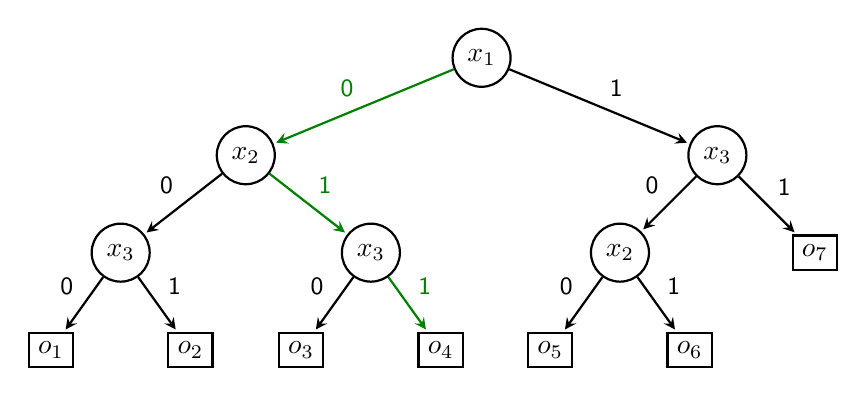
\begin{tikzpicture}[->,>=stealth,shorten >=1pt,auto,node distance=1.75cm, thick,main node/.style={scale=0.9,circle,draw,font=\sffamily\normalsize}]

        \node[circle, draw] (1)[] {$x_1$};

        \node[circle, draw] (2) [below left of=1, xshift=-50, ]{$x_2$};
        \node[circle, draw] (3) [below right of=1, xshift=50, ]{$x_3$};

        \node[circle, draw] (4) [below left of=2, xshift=-10, ]{$x_3$};
        \node[circle, draw] (5) [below right of=2, xshift=10, ]{$x_3$};
        \node[circle, draw] (6) [below left of=3, ]{$x_2$};
        \node[rectangle, draw] (7) [below right of=3]{$o_7$};

        \node[rectangle, draw] (8) [below left of=4, xshift=10]{$o_1$};
        \node[rectangle, draw] (9) [below right of=4, xshift=-10]{$o_2$};
        \node[rectangle, draw] (10) [below left of=5, xshift=10]{$o_3$};
        \node[rectangle, draw] (11) [below right of=5, xshift=-10]{$o_4$};
        \node[rectangle, draw] (12) [below left of=6, xshift=10]{$o_5$};
        \node[rectangle, draw] (13) [below right of=6, xshift=-10]{$o_6$};

        \path[every node/.style={font=\sffamily\small}]
            (1) edge[swap, color=Green]  node{0} (2)
            (1) edge node{1}(3)

            (2) edge[swap]  node{0} (4)
            (2) edge[color=Green]  node{1}(5)

            (3) edge[swap]  node{0} (6)
            (3) edge  node{1}(7)
            
            (4) edge[swap]  node{0} (8)
            (4) edge  node{1}(9)

            (5) edge[swap]  node{0} (10)
            (5) edge[color=Green]  node{1}(11)

            (6) edge[swap]  node{0} (12)
            (6) edge  node{1}(13)
        ;
    \end{tikzpicture}

    \caption{An example of decision tree of size 13 and depth 3. The computation, shown by the green path, for the input $x \in \{0,1\}^n$ is given by $x = 011$}
\end{figure}

Decision trees give an easier way to describe the computation of an oracle Turing machine: if $M^B$ verifies (or solves) a problem $A$ then the $i$-th query made by the procedure corresponds to a variable $x_i$ for the decision tree where $x_i = 1$ if the query returns a positive result and 0 otherwise. In other words, the computation tree of an oracle Turing machine is actually a decision tree.

\begin{proposition}
    If there is an oracle Turing machine $M^B$ that verifies (or solves) a problem $A$ then there is a decision tree that verifies (or solves) $A$. \unsure{Not sure if it's an if and only if, possibly yes}
\end{proposition}

The above proposition gives a strong result that allows us to characterize black-box \TFNP through decision trees instead of oracles: \textit{any decision tree separation implies a relativized separation}. As in the communication complexity formulation described for the white-box model, given a \TFNP problem $R$, we denote with $R^{dt}$ the equivalent $\TFNPdt$ problem, where \textit{dt} stands for \textit{decision tree} \cite{proofs_circuits_communication, tfnp_characterization}.

\begin{definition}
    We define $\mathsf{FP}^{dt}$ as the set of query search problems $R = (R_n)_{n \in \N}$ for which there exists a polylogarithmic depth decision tree $T_n$ such that $T_n(x) = y$ if and only if $(x,y) \in R_n$. Likewise, we define $\mathsf{FNP}^{dt}$ as the set of query search problems $R = (R_n)_{n \in \N}$ for which there exists a polylogarithmic depth decision tree $T_y$ such that $T_y(x) = 1$ if and only if $(x,y) \in R_n$.
\end{definition}

Furthermore, we also introduce the concept of decision tree reductions. Differently from classic and communication search problems, these reductions are based on a more fine-grained definition, where the function that maps inputs of the first problem to inputs of the second problem is computed by many decision trees with output $\{0,1\}$. This definition will allow us to prove some following results in a more convenient way. An analogous formulation can be obtained by computing this function through a simple decision tree. 

\begin{definition}
    A query search problem $R = (R_m)_{m \in \N}$, where $R_m \subseteq \{0,1\}^m \times O_m$ is said to be many-to-one reducible to a query search problem $S = (S_n)_{n \in \N}$, namely $R \leq S$, where $S_n \subseteq \{0,1\}^n \times O_n'$, if for all $m \in \N$ there is an $n \in \N$ for which there is a family of decision trees $T_i : \{0,1\}^m \to \{0,1\}$ for each $i \in [n]$ and a decision tree $T_y^o : \{0,1\}^m \to O_m$ for each $y \in O_n'$ such that:
    \[\forall x \in \{0,1\}^m \;\; (T(x), y) \in S \implies (x, T_y^o(x)) \in R\]
    where $T(x) := (T_1(x), \ldots, T_n(x))$. In other words, the decision trees $T_1, \ldots, T_n$ map inputs of $R$ into inputs of $S$, while the decision tree $g$ maps solutions of $S$ into solutions of $R$. 
\end{definition}

The difference in notation between $T_1, \ldots, T_n$ and $T_y^o$ underlines the fact that the former give a $\{0,1\}$ output, while the latter gives a more output in $O_n$. The \textit{size} of the reduction is the number of input bits to $S$, that being $n$. The \textit{depth} $d$ of the reduction is the maximum depth of any tree involved in the reduction, including each $T_i$ and each $T_y^o$. The \textbf{complexity of the reduction} is given by $\log n + d$. Moreover, we denote as $S^{dt}(R)$ the minimum complexity of any decision tree reduction from $R$ to $S$.

\newpage

Using this definition, we can define complexity classes of total query search problems via decision tree reductions: given a total query search problem $S = (S_n)_{n \in \N}$, we re-define the subclass of problems \textbf{efficiently reducible to $S$} as:
\[S^{dt} := \{R : S^{dt}(R) = \mathrm{polylog}(n)\}\]
where $R = (R_m)_{n \in \N}$.

\section{Connections to Proof Complexity}

Like in the white-box case, the black-box \TFNP model can be studied under multiple lenses. In particular, a well known result extensively discusses even before the rise of the black-box model is the connection between total query search problems and \textbf{propositional proof complexity} \cite{tfnp_characterization, separations_proof_complexity,proofs_circuits_communication}.

\improvement{Add proof complexity discussion here or in preliminaries}

It's easy to see that any CNF formula gives rise to an associated search problem: finding an unsatisfied clause inside the formula (if there is any).

\begin{definition}
    Given the CNF $F = C_1 \land \ldots \land C_m$ over $n$ variables, we define  $\mathrm{Search}(F)$ as the following associated search problem: given an input assignment $\alpha(x_1, \ldots, x_n)$, return the index of an unsatisfied clause (if there is any).
\end{definition}

In particular, when $F$ is an unsatisfiable CNF formula, $\mathrm{Search}(F)$ is clearly a \textit{total search problem} since for any input assignment there will always be an unsatisfied clause. In a similar fashion, we can show that any total query search problem $R$ can be associated with the search problem of the formula $F$ that describes the set of decision trees that verify $R$.

Consider a decision tree $T$ made of the paths $p_1, \ldots, p_k$, each leading to the leaves $\ell_1, \ldots, \ell_k$. The DNF encoding of $T$, denoted with $D_T$, is the disjunction over the conjunction of the literals $\alpha_1, \ldots, \alpha_h$ along each of the accepting paths in $T$. In other words, we have that $D_T = p_1 \lor \ldots \lor p_k$ where each $p_i = \alpha_1 \land \ldots \land \alpha_h \land \ell_i$ is an accepting path of $T$. We notice that, by De Morgan's theorem, $\lnot{D_T}$ is a CNF.

\begin{proposition}
    \label{Rdt = Search(F)}
    Given a total query search problem $R \subseteq \{0,1\}^n \times O$, for each $n \in \N$ there exists an unsatisfiable CNF formula $F_n$ defined over $\abs{O}$-many variables such that $R_n = \mathrm{Search}(F_n)$. This formula is called canonical CNF encoding of $R_n$.
\end{proposition}

\begin{proof}
    Since $R = (R_n)_{n \in \N} \in \TFNP^{dt}$, for each $y \in O_n$ there is a $\mathrm{polylog}(n)$-depth decision tree $T_y$ that verifies $R_n$. Consider the CNF $F_n := \bigwedge\limits_{y \in O_n} \lnot{D_{T_y}}$. Since $R$ is a total search problem, for each input $x$ there is a valid output, implying that at least one tree $T_y$ will have an accepting path, meaning that $D_{T_y}(x) = 1$ and therefore $\lnot{D_{T_y}}(x) = 0$, concluding that $F_n$ is unsatisfiable. Moreover, this formulation also concludes that:
    \[(x,y) \in R_n \iff T_y(x) = 1 \iff \lnot{D_{T_y}}(x) = 0 \iff (x,y) \in \mathrm{Search}(F_n)\]
    and thus that $R_n = \mathrm{Search}(F_n)$.

\end{proof}

This result clearly implies that $(R)_{n \in \N} = (\mathrm{Search}(F_n))_{n \in \N}$, where $F_1, F_2, \ldots$ is a family of CNF formulas, and by extension that black-box \TFNP is \textit{exactly} the study of the false clause search problem. Like in the white-box case, the upshot is that it is sufficient to restrict our interests on the study of search problems associated to unsatisfiable CNF formulas.

Through this connection, Göös et al. \cite{adventures_monotone_tfnp} showed that many important proof systems are characterized by an associated $\TFNPdt$ search problem and vice versa. 

Given a proof system $P$ and an unsatisfiable CNF formula $F$, the \textbf{complexity} required by $P$ to prove $F$ is given by:
\[P(F) := \min\{\log \mathrm{size}(\Pi) + \mathrm{deg}(\Pi) : \Pi \text{ is a $P$-proof of } F\}\]
where $\mathrm{size}(\Pi)$ is the \textit{size} of $\Pi$ in $P$, i.e. the sum of the sizes of all the formulas inside it or in other words the total number of symbols in $\Pi$, and $\mathrm{deg}(\Pi)$ is the \textit{degree} of $\Pi$ associated to $P$, which varies from proof system to proof system. This degree measure will be specified for the proof systems used in following sections.

Since each $\TFNPdt$ problem is equivalent to the false clause search problem of a family $F$ of formulas, the complexity parameter defined above can be used to define another characterization of $\TFNPdt$ problems.

\begin{definition}
    We say that a proof system $P$ \textbf{characterizes} a $\TFNPdt$ problem $R$ (and reflexively that $R$ characterizes $P$) if it holds that \[R^{dt} = \{\mathrm{Search}(F) : P(F) = \mathrm{polylog}(n)\}\]
    where $F = F_1, F_2, \ldots$ is a family of formulas. In a stronger sense, it holds that $R^{dt}(\mathrm{Search}(F)) = \Theta(P(F))$.
\end{definition}

Most of the \TFNP subclasses discussed in previous sections has been shown to have a characterizing proof system. References and proofs to these characterizations can be found in \cite{separations_proof_complexity,tfnp_characterization}.
\begin{itemize}
    \item $\mathrm{PLS}^{dt}(\mathrm{Search}(F)) = \Theta(\mathrm{TreeRes}(F))$
    \item $\mathrm{PPA}^{dt}(\mathrm{Search}(F)) = \Theta(\F_2\mathrm{-NS}(F))$
    \item $\mathrm{PPADS}^{dt}(\mathrm{Search}(F)) = \Theta(\mathrm{unary-NS}(F))$
    \item $\mathrm{PPAD}^{dt}(\mathrm{Search}(F)) = \Theta(\mathrm{unary-SA}(F))$
    \item $\mathrm{SOPL}^{dt}(\mathrm{Search}(F)) = \Theta(\mathrm{RevRes}(F))$
    \item $\mathrm{CLS}^{dt}(\mathrm{Search}(F)) = \Theta(\mathrm{RevResT}(F))$
    \item $\mathrm{FP}^{dt}(\mathrm{Search}(F)) = \Theta(\mathrm{TreeRes}(F))$
\end{itemize}

\newpage

\section{Canonical Proof Systems}

In an intuitive way, this characterization also shows that \textit{any} $\TFNPdt$ problem can be transformed into a proof system for refuting unsatisfiable CNF formulas of polylogarithmic width: since any $\TFNPdt$ is equivalent to the search problem for some unsatisfiable CNF formula, any efficient decision tree reduction between problems is nothing more than an efficient proof in the characterizing proof system and vice versa. To formalize this idea, we introduce the concept of \textbf{reductions between CNF formulas} \cite{tfnp_characterization}.

Suppose that $C$ is a clause over $n$ variables and that $T = (T_i)_{i \in [n]}$ is a sequence of depth-$d$ decision trees, where $T_i : \{0,1\}^{n'} \to \{0,1\}$. We refer to $C(T)$ as the CNF formula obtained by substituting each variable $x_i$ in $C$ with the associated tree $T_i$ and rewriting the result as a CNF, or more conveniently:
\[C(T) := \bigwedge_{i \in [n]} \, \bigwedge_{\substack{r \,:\, \text{rejecting} \\ \text{path of $T_i$}}} \overline{r}\]

\begin{definition}
    Let $F = C_1 \land \ldots \land C_{m_F}$ be an unsatisfiable CNF over $n_F$ variables. We say that a CNF formula $H$ made of $m_H$ clauses over $n_H$ variables reduces to $F$ via depth-$d$ decision trees if there exist two sequences of depth-$d$ decision trees $T = (T_i)_{i \in [n_F]}$ and $T' = (T_j^o)_{j \in [m_F]}$, where $T_i : \{0,1\}^{n_H} \to \{0,1\}$ and $T_j^o : \{0,1\}^{n_H} \to [m_H]$, such that given the following formula:
    \[F_H := \bigwedge_{j \in [m_F]} \,\bigwedge_{\substack{p \,:\; \text{path} \\ \text{in } T_j^o}} C_i(T) \lor \overline{p}\]
    it holds that if $F$ is unsatisfiable then $F_H$ is unsatisfiable and by consequence that $H$ is unsatisfiable. 
\end{definition}

In particular, we notice that $F_H$ can also be written as a CNF by simply distributing each $\overline{p}$ inside $C_i(T)$. Each clause $C_i(T) \lor \overline{p}$ must be either tautological (since it could contain a variable and its negation) or a weakening of the corresponding clause of $H$ indexed by the label at the end of the path $p$. Moreover, we notice that through this formulation any depth-$d$ decision tree reduction from $\mathrm{Search}(H)$ to $\mathrm{Search}(F)$ induces the search problem $\mathrm{Search}(F_H)$.

Reductions between CNF formulas imply that reductions between search problems reduction are actually a proof system. In particular, given a problem $\mathrm{Search}(F) \in \TFNPdt$, the \textbf{canonical proof system} of such problem, denoted with $P_F$ proves an unsatisfiable formula $H$ over $n_H$ variables if $H$ is reducible to an instance of $F$ over $n_F$ variables. A $P_F$-proof of $H$ consists of the decision trees that make such reduction possible. The \textit{size} of such proof is given by $n_F$, while the \textit{degree}, or \textit{depth} in this case, is given by the maximum depth among the involved decision trees. Hence, the $P_F$ complexity of $H$ is given by:
\[P_F(H) := \min\{\log n_H + \mathrm{depth}(\Pi) : \Pi \text{ is a $P_F$-proof of } H\}\]

These proof systems are \textit{sound}, since by construction any valid substitution of an unsatisfiable CNF formula is also unsatisfiable, and also \textit{efficiently verifiable}, since it suffices to check that each of the clauses of $F_H$ is either tautological or a weakening of a clause in $H$, which can be done polynomially in size of the proof.

From this definition of canonical proof system, the following theorem is given for free. This theorem plays a crucial role in $\TFNPdt$ characterization through proof complexity, stating that $P_F$ has a short proof of $H$ if and only if $\mathrm{Search}(H)$ efficiently reduces to $\mathrm{Search}(F)$. 

In particular, we observe that \textbf{any characterizing proof system} is actually the canonical proof system of the associated search problem, a result that follows from the two definitions. In other words, proving a formula in a characterizing proof system automatically gives a reduction to the corresponding complete search problem.

\begin{theorem}
    Let $\mathrm{Search}(F) \in \TFNPdt$ and let $H$ be an unsatisfiable CNF formula. The two following results hold:
    \begin{enumerate}
        \item If $H$ has a size $s$ and depth $d$ proof in $P_F$ then $\mathrm{Search}(H)$ has a size $O(s)$ and depth $d$ reduction to $S_F$
        \item If $\mathrm{Search}(H)$ has a size $s$ and depth $d$ decision tree reduction to $\mathrm{Search}(F)$ then $H$ has a size $s2^{O(d)}$ and depth $d$ proof in $P_F$
    \end{enumerate}
    In particular, this implies that $\mathrm{Search}(F)^{dt}(\mathrm{Search}(H)) = \Theta(P_F(H))$.
\end{theorem}

\begin{proof}
    Suppose that $T = (T_i)_{i \in [n_F]}$ and $T' = (T_j^o)_{j \in [m_F]}$ is a $P_F$ proof of $H$ of size $s$ and depth $d$. Given any assignment $x$ such that $(x, i) \in \mathrm{Search}(F)$, let $C_i$ be the clause of $F$ falsified by $T_1(x), \ldots, T_{n_F}(x)$ and let $p$ be the path followed by $T_i^o(x)$. It's easy to see that a clause of the formula $C_i(T) \lor \overline{p}$ must be falsified by $x$. In particular, such clause is also the weakening of the $T_i^o(x)$-th clause of $H$, concluding that $(x, T_i^o(x)) \in \mathrm{Search}(H)$. In other words, the $P_F$ proof of $H$ corresponds to a reduction from $\mathrm{Search}(H)$ to $\mathrm{Search}(F)$ of size $n_F = O(s)$ and depth $d$.

    Vice versa, suppose that $T = (T_i)_{i \in [n_F]}$ and $T' = (T_j^o)_{j \in [m_F]}$ is a decision tree reduction from $\mathrm{Search}(H)$ to $\mathrm{Search}(F)$ of size $s$ and depth $d$. Then, we can construct $F_H$ as previously described through the use of these decision trees. Let $L$ be a clause of $C_i(T)$ for some $i \in [m_F]$ and let $p$ be any path in $T_i^o$. If the formula $C_i(T) \lor \overline{p}$ is tautological, then it can be ignored since $F_H$ is a CNF. Otherwise, let $x$ be an assignment that falsifies $L \lor \overline{p}$. Then, it holds that $T_1(x), \ldots, T_{n_F}(x)$ falsifies $C_i(T)$ and that $T_i^o(x)$ follows path $p$. Thus, the $T_i(x)$-th clause of $\overline{H}$ must also be false, implying that $L \lor \overline{p}$ is a weakening of such clause. This concludes that $F_H$ is a $P_F$-proof of $H$ of depth at most $d$ (due to how $F_H$ is constructed) and thus that the size is at most $s2^{O(d)}$.

\end{proof}

\cleardoublepage